\documentclass[10pt]{article}
\usepackage[utf8]{inputenc}
\usepackage{setspace}
\doublespacing
\usepackage{lipsum} 
\usepackage[margin=1in]{geometry}
%\usepackage{mathptmx}
%\setlength\parindent{0pt}
\usepackage{fancyhdr}
%\usepackage{natbib}
\usepackage{indentfirst}
\usepackage{subcaption}
\usepackage{graphicx}
\usepackage{amssymb} %maths
\usepackage{amsmath} %maths

\begin{filecontents}{ref2.bib}
@article{large_scale_english,
   title={Large-Scale Analysis of Zipf’s Law in English Texts},
   volume={11},
   ISSN={1932-6203},
   url={http://dx.doi.org/10.1371/journal.pone.0147073},
   DOI={10.1371/journal.pone.0147073},
   number={1},
   journal={PLOS ONE},
   publisher={Public Library of Science (PLoS)},
   author={Moreno-Sánchez, Isabel and Font-Clos, Francesc and Corral, Álvaro},
   editor={Chialvo, Dante R.Editor},
   year={2016},
   month={1},
   pages={e0147073}
}

@article{seven_lang,
   title={Universal and non-universal text statistics: Clustering coefficient for language identification},
   ISSN={0378-4371},
   url={http://dx.doi.org/10.1016/j.physa.2019.123905},
   DOI={10.1016/j.physa.2019.123905},
   journal={Physica A: Statistical Mechanics and its Applications},
   publisher={Elsevier BV},
   author={Espitia, Diego and Larralde, Hernán},
   year={2019},
   month={12},
   pages={123905}
}

@inproceedings{esperanto,
    author = {Manaris, Bill and Pellicoro, Luca and Pothering, George and Hodges, Harland},
    year = {2006},
    month = {02},
    pages = {102-108},
    title = {Investigating Esperanto's Statistical Proportions Relative to other Languages using Neural Networks and Zipf's Law.},
    journal = {Proceedings of the IASTED International Conference on Artificial Intelligence and Applications, AIA 2006}
}

@article{fifty_lang,
    author = {Yu, Shuiyuan and Xu, Chunshan and Liu, Haitao},
    year = {2018},
    month = {07},
    pages = {},
    title = {Zipf's law in 50 languages: its structural pattern, linguistic interpretation, and cognitive motivation}
}

@article{taylor_zipf,
author = {Belevitch, Vitold},
year = {1959},
month = {01},
pages = {},
title = {On the statistical laws of linguistic distributions},
volume = {173},
journal = {Annales de la Société Scientifique de Bruxelles. Série I}
}

% Cambridge, Mass.: Addison-Wesley Press, Inc., 1949. 573 pp. \\ \$6.50
@article{zipf,
    author = {Zipf, George},
    title = "{Human Behavior and the Principle of Least Effort: An Introduction to Human Ecology}",
    journal = {Social Forces},
    volume = {28},
    number = {3},
    pages = {340-341},
    year = {1950},
    month = {03},
    issn = {0037-7732},
    doi = {10.2307/2572028},
    url = {https://doi.org/10.2307/2572028},
    eprint = {https://academic.oup.com/sf/article-pdf/28/3/340/5861620/28-3-340.pdf},
}

@article{not_random_words_zipf,
    author = {Ferrer-i-Cancho, Ramon AND Elvevåg, Brita},
    journal = {PLOS ONE},
    publisher = {Public Library of Science},
    title = {Random Texts Do Not Exhibit the Real Zipf's Law-Like Rank Distribution},
    year = {2010},
    month = {03},
    volume = {5},
    url = {https://doi.org/10.1371/journal.pone.0009411},
    pages = {1-10},
    number = {3},
    doi = {10.1371/journal.pone.0009411}
}

@article{random_words_zipf,
    author = {Li, W.},
    title = {Random Texts Exhibit Zipf’s-Law-like Word Frequency Distribution},
    year = {2006},
    issue_date = {November 1992},
    publisher = {IEEE Press},
    volume = {38},
    number = {6},
    issn = {0018-9448},
    url = {https://doi.org/10.1109/18.165464},
    doi = {10.1109/18.165464},
    journal = {IEEE Trans. Inf. Theor.},
    month = sep,
    pages = {1842–1845},
    numpages = {4}
}

@misc{graph,
    title={Phase transitions in a decentralized graph-based approach to human language},
    author={Javier Vera and Felipe Urbina and Wenceslao Palma},
    year={2020},
    eprint={2003.02639},
    archivePrefix={arXiv},
    primaryClass={physics.soc-ph}
}

@inproceedings{physics,
author = {Wang, Qiuping},
year = {2020},
month = {02},
pages = {},
title = {Deriving Zipf's law: principle of least effort vs. maximum efficiency}
}

@misc{earthquake,
    title={Zipf-Mandelbrot Law for Time Intervals of Earthquakes},
    author={Sumiyoshi Abe and Norikazu Suzuki},
    year={2002},
    eprint={cond-mat/0208344},
    archivePrefix={arXiv},
    primaryClass={cond-mat.dis-nn}
}

@article{music,
author = {Damiáan H. Zanette},
title ={Zipf's law and the creation of musical context},
journal = {Musicae Scientiae},
volume = {10},
number = {1},
pages = {3-18},
year = {2006},
doi = {10.1177/102986490601000101},
URL = {https://doi.org/10.1177/102986490601000101}
}

@misc{impersonation,
    title={Domain-based Latent Personal Analysis and its use for impersonation detection in social media},
    author={Osnat Mokryn and Hagit Ben-Shoshan},
    year={2020},
    eprint={2004.02346},
    archivePrefix={arXiv},
    primaryClass={cs.CL}
}


@online{Moby-Dick,
    author = {Melville, Herman},
    title = {Moby-Dick; or, The Whale},
    place = {Urbana, Illinois},
    url = {https://www.gutenberg.org/files/2701/2701-h/2701-h.htm},
    publisher = {Project Gutenberg},
    year = {2008},
    urldate = {2020-04-20}
}

@online{Ulysses,
    author = {Joyce, James},
    title = {Ulysses},
    place = {Urbana, Illinois},
    url = {https://www.gutenberg.org/files/4300/4300-h/4300-h.htm},
    publisher = {Project Gutenberg},
    year = {2008},
    urldate = {2020-04-20}
}

@article{trump,
    author     = {TIME Staff},
    title      = {Donald Trump's Interview With TIME on 2020: Read the Transcript},
    journal    = {TIME Magazine},
    year       = 2019,
    url = {https://time.com/5611476/donald-trump-transcript-time-interview/}
}

@online{capone,
    title = {Al Capone Trial: Selected Documents: Interview of Al Capone (April 17, 1931)},
    author = {Capone, Al},
    url = {http://law2.umkc.edu/faculty/projects/ftrials/capone/caponeinterview.html},
    year = {1931},
    urldate = {2020-04-20}
}

@online{paradiselost,
    title = {Paradise Lost: Book  1 (1674 version)},
    author = {Milton, John},
    url = {https://www.poetryfoundation.org/poems/45718/paradise-lost-book-1-1674-version},
    year = {1674},
    urldate = {2020-04-20}
}

@online{feynman,
    title = {The Feynman Lectures on Physics, Volume I},
    author = {Feynman, Richard and Leighton, Robert and Sands, Matthew},
    url = {https://www.feynmanlectures.caltech.edu/I_toc.html},
    year = {1963},
    urldate = {2020-04-20}
}
\end{filecontents}

\usepackage[american]{babel}
\usepackage{csquotes}
\usepackage[style=apa,backend=biber]{biblatex}
\DeclareLanguageMapping{american}{american-apa}
\addbibresource{ref2.bib}

\setlength\parindent{10in}

\title{On the Existence and Cause of Zipf's Law}
\author{Elijah Sheridan}

\begin{document}

\pagestyle{fancy}
\rhead{\thepage}  % Page number in header
\cfoot{}

\setlength{\abovedisplayskip}{4pt}
\setlength{\belowdisplayskip}{4pt}

\begin{titlepage}
	\centering
	\vspace*{2.75cm}
	{\scshape \LARGE \textbf{On the Existence of Zipf's Law and Its Potential Origins in Statistics or Optimization} \par}
	\vspace*{1.25cm}
	{Elijah Sheridan \par}
	
	{Department of Psychology and Human Development, Vanderbilt University \par}
	
	{PSY-PC 3130: Introduction to Formal Linguistics \par}

	{Dr. Duane Watson \par}

	{April 20, 2020 \par}
\end{titlepage}

\begin{flushleft}
    \hspace*{0.5in} When considering language samples---such as works of literature, conversations, or textbooks, to name a few classes of examples---one can make reasonable estimations and generalizations about their word content. Considering samples from the English corpus in particular, one would likely predict, for example, to see small sets of words used a lot---function words like ``the,'' ``to,'' and ``with''---and a larger set of words used less frequently, like nouns and adjectives. While many native speakers have these loose intuitions, the non-trivial linguistics question is then if anything more precise and perhaps mathematical can be said about word frequencies within given texts in general. In this paper, I seek to investigate and explore this inquiry. In particular, I intend to show that, across languages, a notable portion of samples obey what is called Zipf's law---named after Harvard linguist George Zipf, who popularized the idea---which states that the relative frequency of a word in a text is proportional to the reciprocal of its position when ranked among all words in that text by frequency. My exposition of this effect will then be followed by a discussion of the potential origination of this global phenomenon: this remains an open question, but compelling arguments have been constructed using both statistical and optimization approaches. I will personally advocate for the latter of these options, as a consequence of its generality and compatibility with broader scientific principles, in particular those appearing in physics.
    
    \hspace*{0.5in} I begin by more formally defining Zipf's law as it appears in language, which will enable an argument its existence there and a more thorough treatment of the principle in the following sections. Letting $S$ denote the set of words appearing in a given language sample, ordered by frequency such that the word $s_i$ in $S$ is the $i$th most frequently used word in the sample, I use $N_i$ to denote the precise number of times $s_i$ appears. If there are $N$ words in our body, then the probability $p_i$ of an arbitrary word in the text being $s_i$ is then $\frac{N_i}{N}$. The motivating question posed about the nature of the relative frequencies of words can then be understood as a question about the behavior of $p_i$, and perhaps its relationship to $i$, the rank. Zipf's law is the claim that $p_i$ and $i$ obey the following relationship, letting $p_1$ denote the probability of the most common word in the sample.
    \begin{equation}
        \frac{p_i}{p_1} \propto \frac{1}{i^\alpha} \label{eq:zipf}
    \end{equation}
    It's worth noting that this is really a class of relationships, rather than a particular one, as $\alpha$ is a variable and different choices for its value result in different behaviors. However, if $\alpha \approx 1$---as it often is, something I will soon provide evidence for---then we can understand Zipf's law as the following statement: the most frequent word in a text appears $i$ times as often as the $i$th most frequent word. This would mean that relative word frequency is quite hierarchical: Zipf's law asserts that there aren't sets of words which are all used approximately the same amount in given texts, but rather that a pecking order of words emerges, and one that is particularly evident in the high frequency domain (as $\frac{1}{i^\alpha}$ and $\frac{1}{(i+1)^\alpha}$ are further apart for small $i$).
    
    \hspace*{0.5in} Having more rigorously established the content of Zipf's law, I now turn my attention to actually exhibiting its presence in language. However, at first glance, the task of quantitatively assessing whether or not a body of language adheres to Eq. \ref{eq:zipf} is not an easy one. A simple solution, though, can be achieved by transforming this problem into one of linear regression, enabling the use of classical statistical methods. This can be arranged through the following manipulation of Eq. \ref{eq:zipf} using properties of the natural logarithm, where $c$ is a proportionality constant.
    \begin{equation}
        \frac{p_i}{p_1} = \frac{c}{i^\alpha} \;\; \Longrightarrow \;\; \ln\left(\frac{p_i}{p_1}\right) = \ln\left(\frac{c}{i^\alpha}\right) \;\; \Longrightarrow \;\; \ln(p_i) = -\alpha\ln(i) + \ln(c \cdot p_1) \label{eq:log}
    \end{equation}
    It follows that Zipf's law implies a linear correlation between the variables $\ln(p_i)$ and $\ln(i)$ with a slope of $-\alpha \approx -1$, allowing us assess a sample's agreement with Zipf's law by computing these parameters for each word, performing linear regression, and considering the resulting coefficient of determination $r^2$. I've completed this process for six bodies of language: two novels, \textcite{Moby-Dick} and \textcite{Ulysses}; a poem, \textcite{paradiselost}; two interviews, \textcite{trump} and \textcite{capone}; and the first $20$ lectures from \textcite{feynman}. My results are summarized in Fig. \ref{fig:plots}. The $\ln(i)$ vs $\ln(p_i)$ plots corresponding to the two novels, the first interview, and the lectures are visibly linear and the corresponding linear regressions satisfy $r^2 > 0.96$, which is interpreted as $96\%$ of the variation in $\ln(p_i)$ being explained by a linear relationship with $\ln(i)$. This points to Zipf's law holding across different forms of language, from literature to conversation to instruction. Moreover, we encounter $\alpha \approx 1$ (with some exception occurring for the Feynman lectures) as I earlier alluded to. The final two sources, with their lower $r^2$ values and less linear plots, are included as counterexamples to demonstrate that Zipf's law doesn't hold perfectly in all cases: the lexcial uniqueness of works of poetry like \textcite{paradiselost} and sheer brevity of \textcite{capone} likely prevent the exhibition of Zipf's law, which as a statistical phenomenon depends upon a certain regularity and word sample size to appear. While it is important to note that some samples don't adhere to Zipf's law, I now want to begin a discussion which will point to the sizeable manifestation of Zipf's law in language.
    
    \begin{figure}[ht]
    \begin{minipage}{0.35\linewidth}
        \centering
        \small
        Text Statistics
        
        \bigskip
        
        \begin{tabular}{@{}*{4}{c}@{}}
            \hline
        Source & $N$ & $r^2$ & $|m|$ \\ 
            \hline
        (a) & $208458$ & $0.972$ & $1.07$ \\
        (b) & $264977$ & $0.968$ & $1.02$ \\
        (c) & $9903$ & $0.972$ & $1.09$ \\
        (d) & $123898$ & $0.969$ & $1.31$ \\
        (e) & $5996$ & $0.908$ & $0.72$ \\
        (f) & $733$ & $0.933$ & $0.82$ \\
            \hline
        \end{tabular}
    \end{minipage}
    \begin{minipage}{0.65\linewidth}
        \begin{subfigure}{0.32\linewidth}
            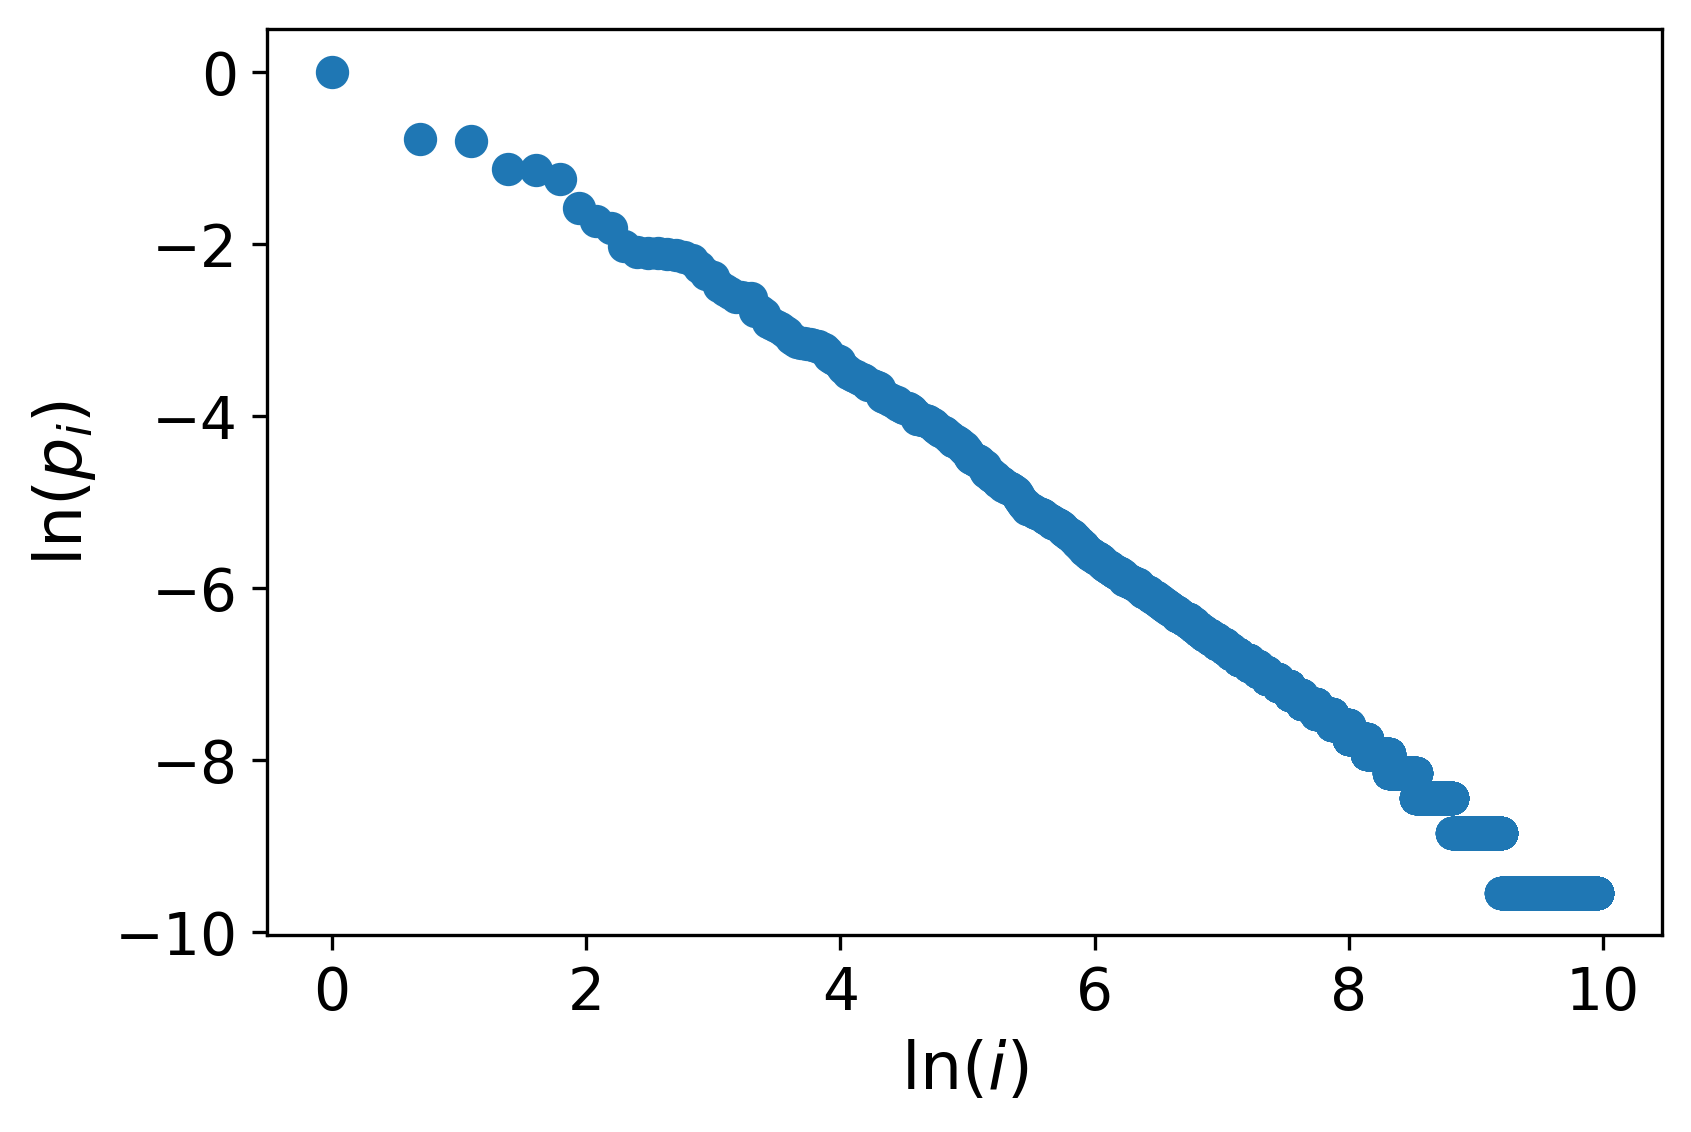
\includegraphics[width=0.99\linewidth]{images/mobydick.png}
            \caption{}
        \end{subfigure}
        \begin{subfigure}{0.32\linewidth}
            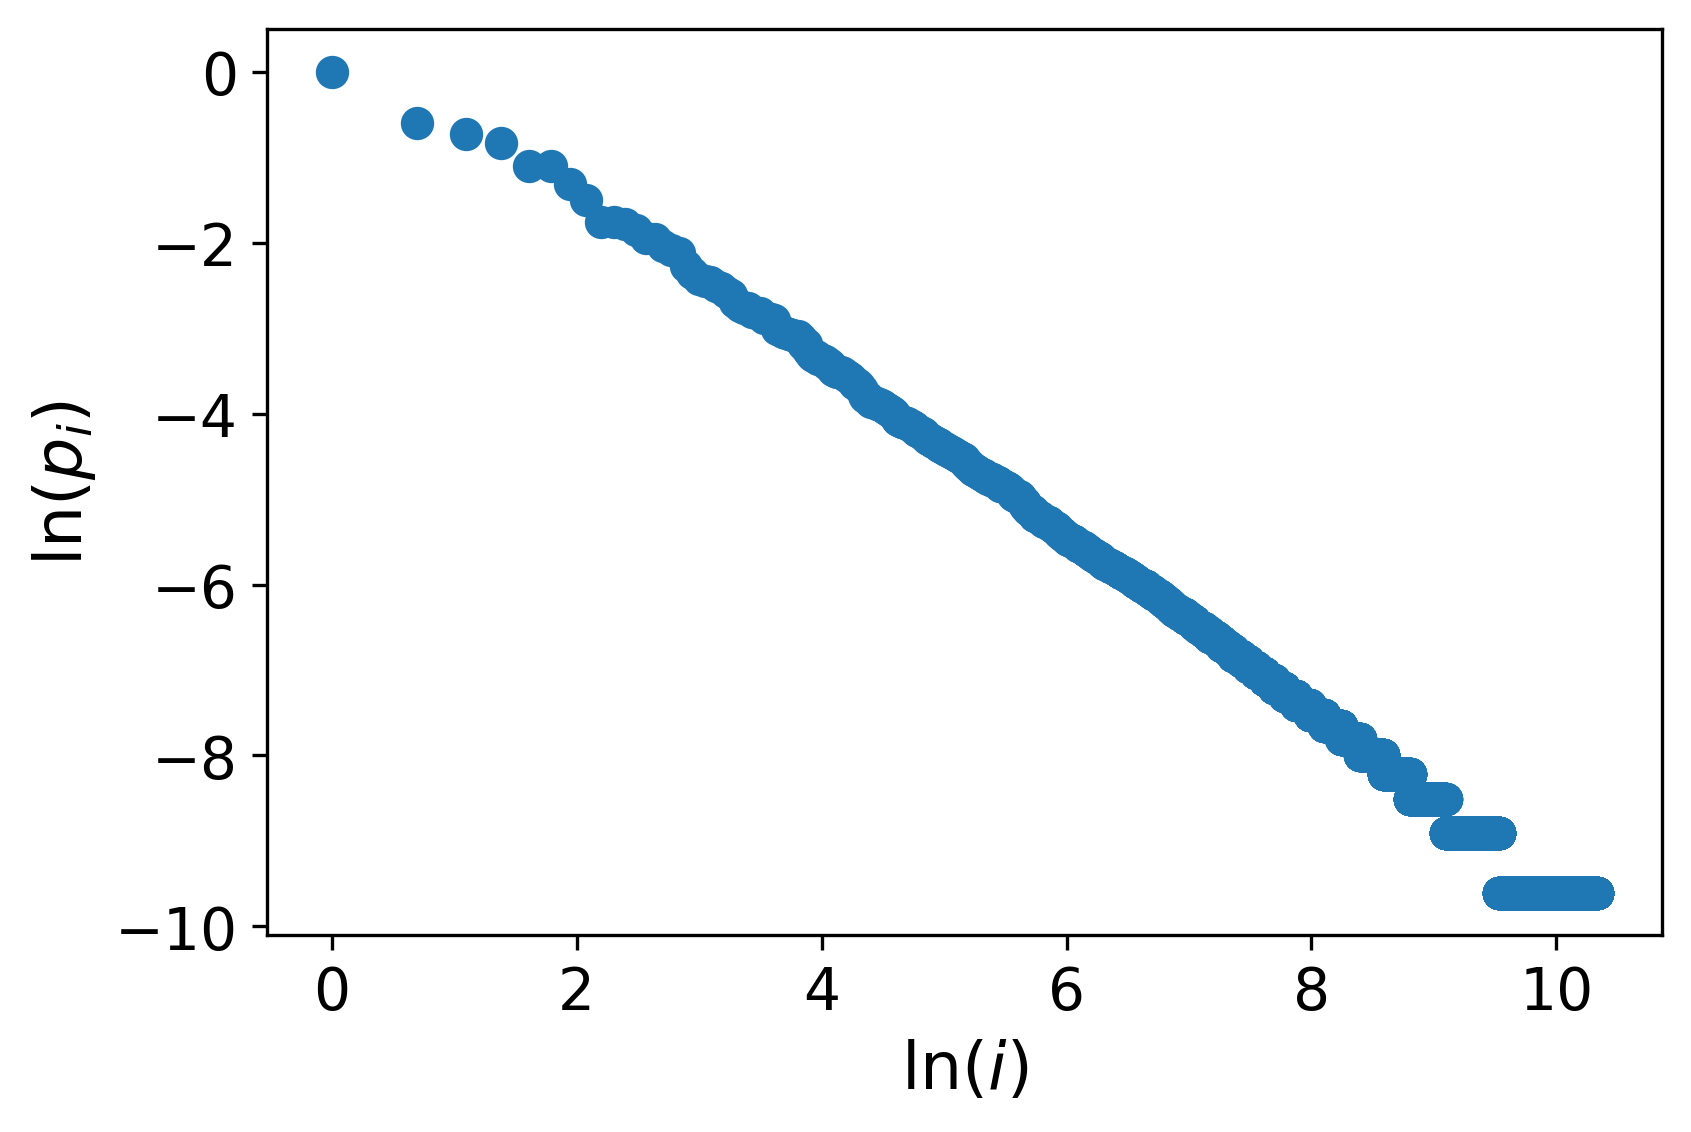
\includegraphics[width=0.99\linewidth]{images/ulysses.png}
            \caption{}
        \end{subfigure}
        \begin{subfigure}{0.32\linewidth}
            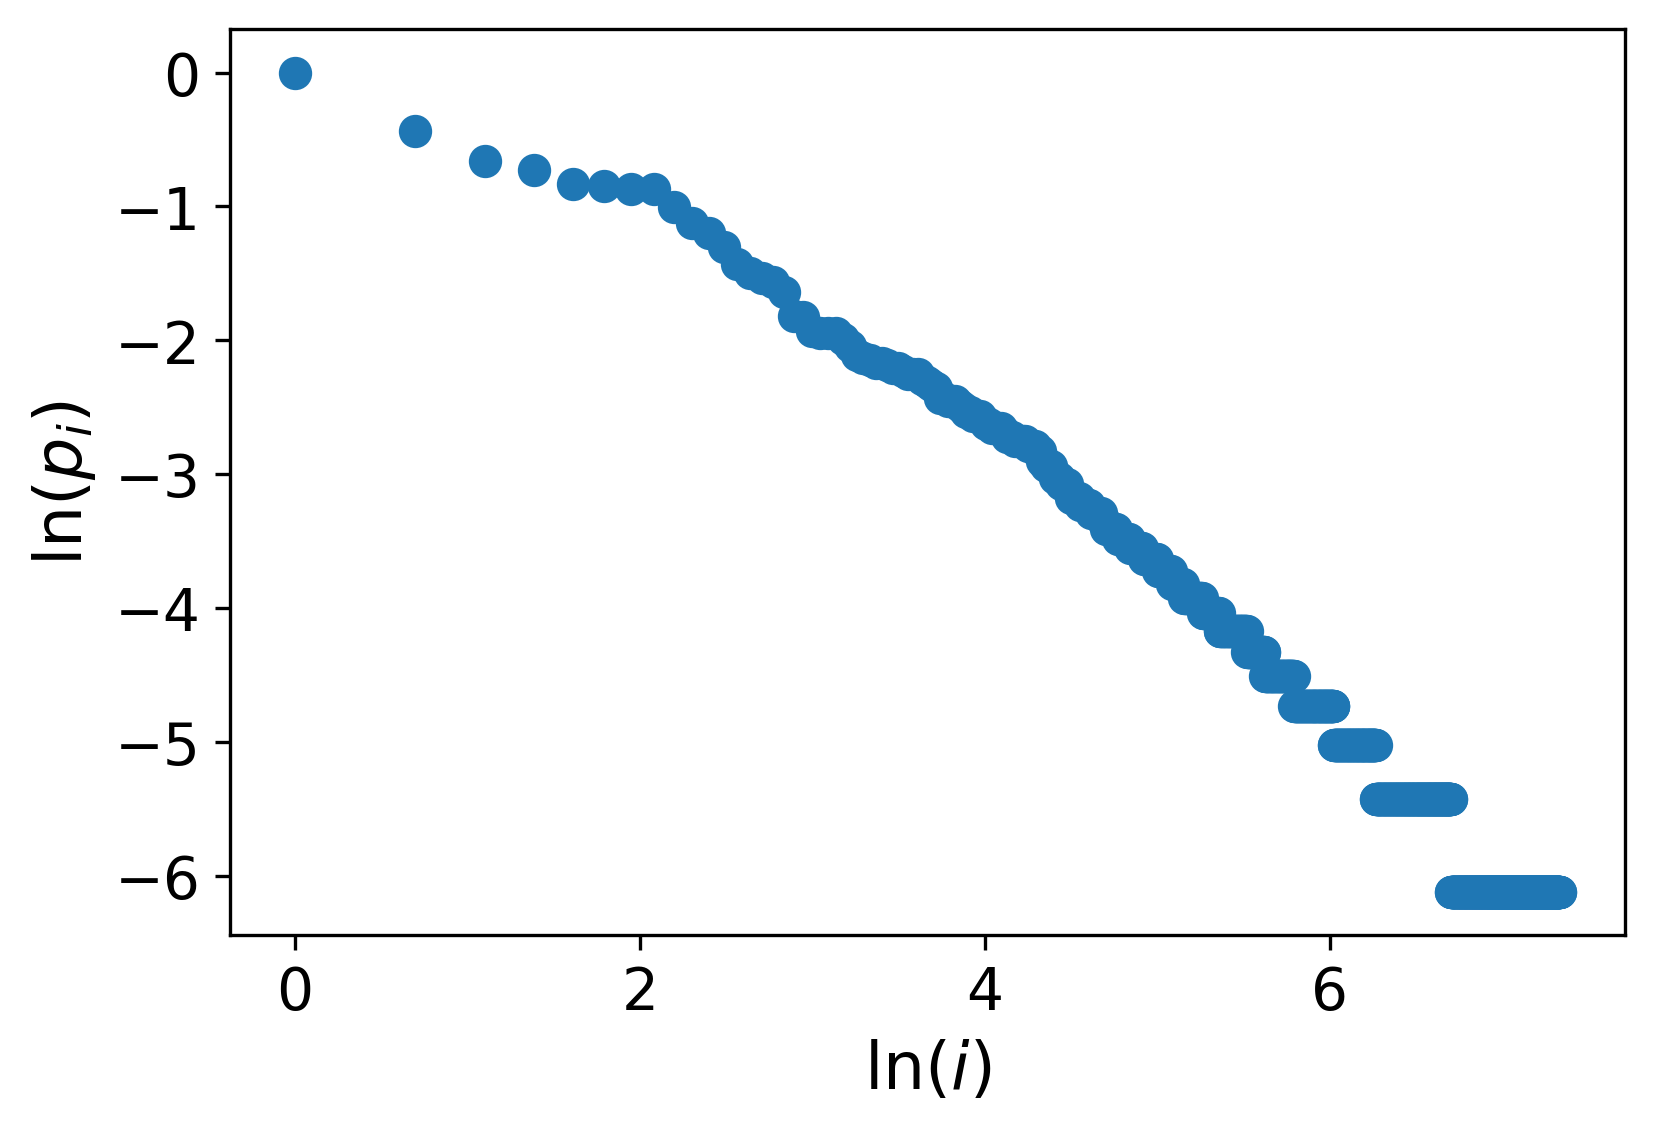
\includegraphics[width=0.99\linewidth]{images/trump.png}
            \caption{}
        \end{subfigure}
        \\
        \begin{subfigure}{0.32\linewidth}
            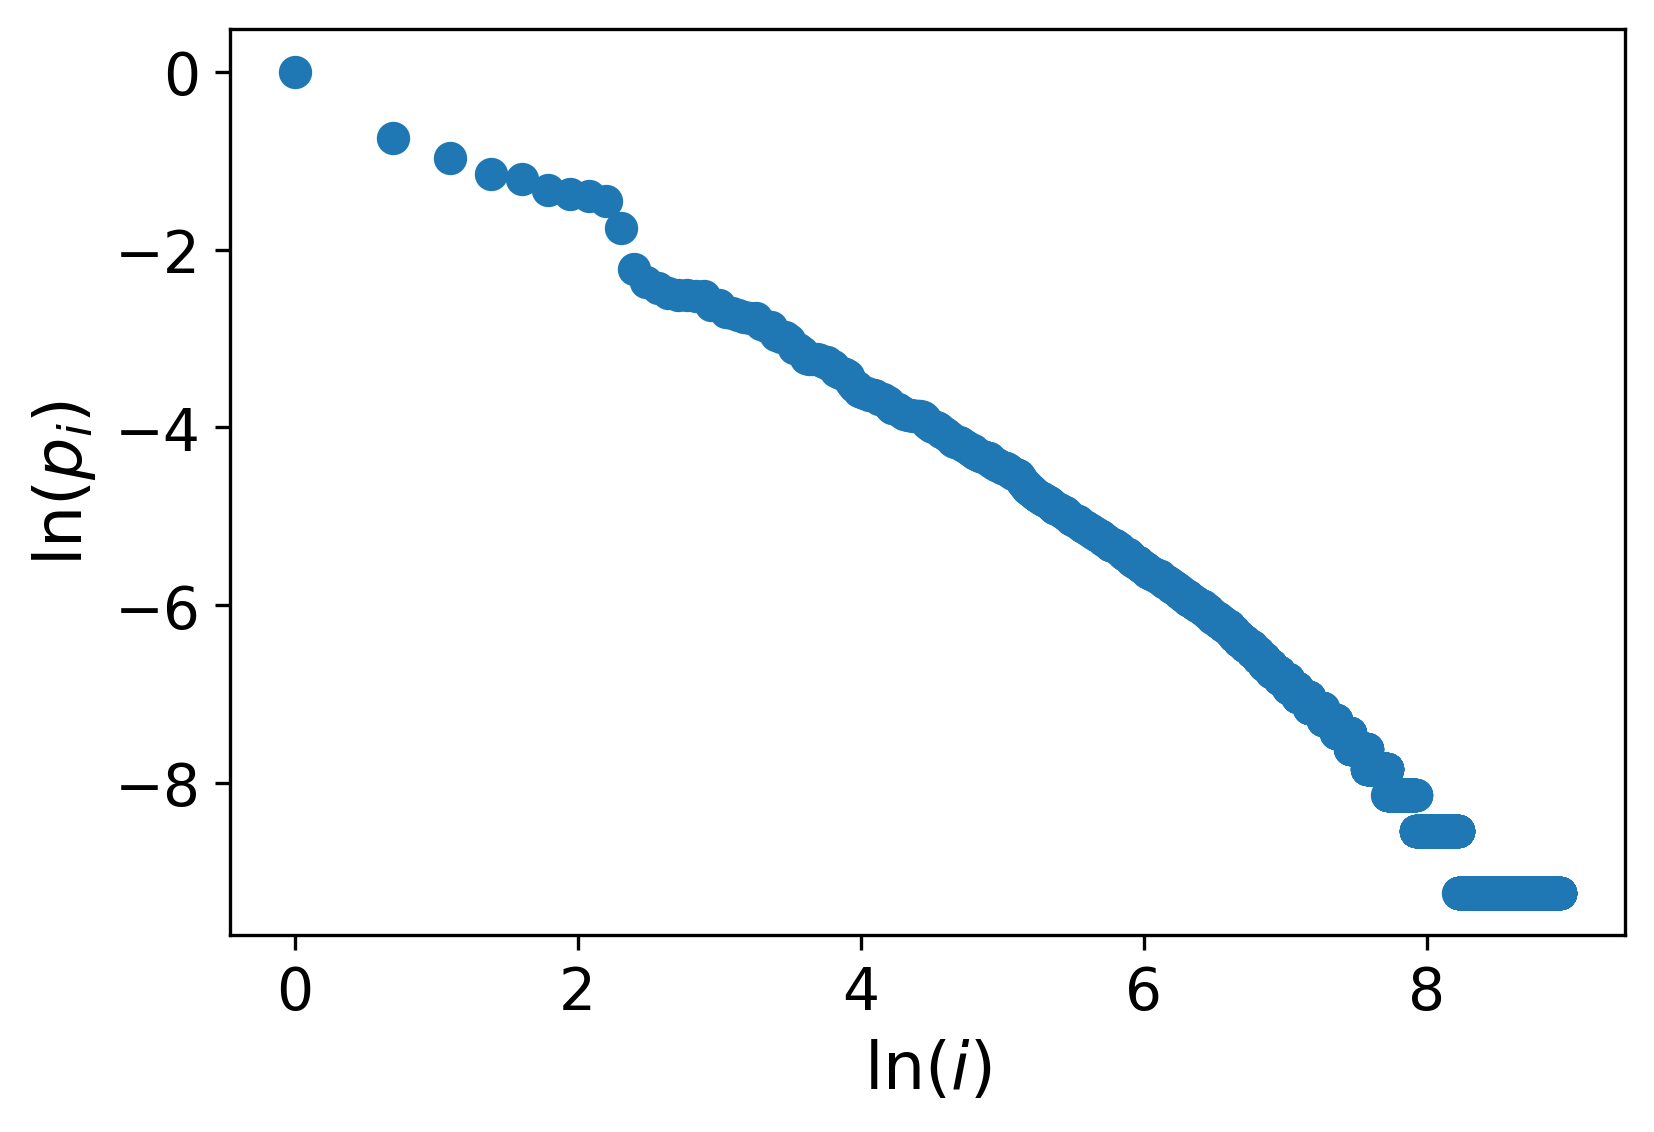
\includegraphics[width=0.99\linewidth]{images/feynmann.png}
            \caption{}
        \end{subfigure}
        \begin{subfigure}{0.32\linewidth}
            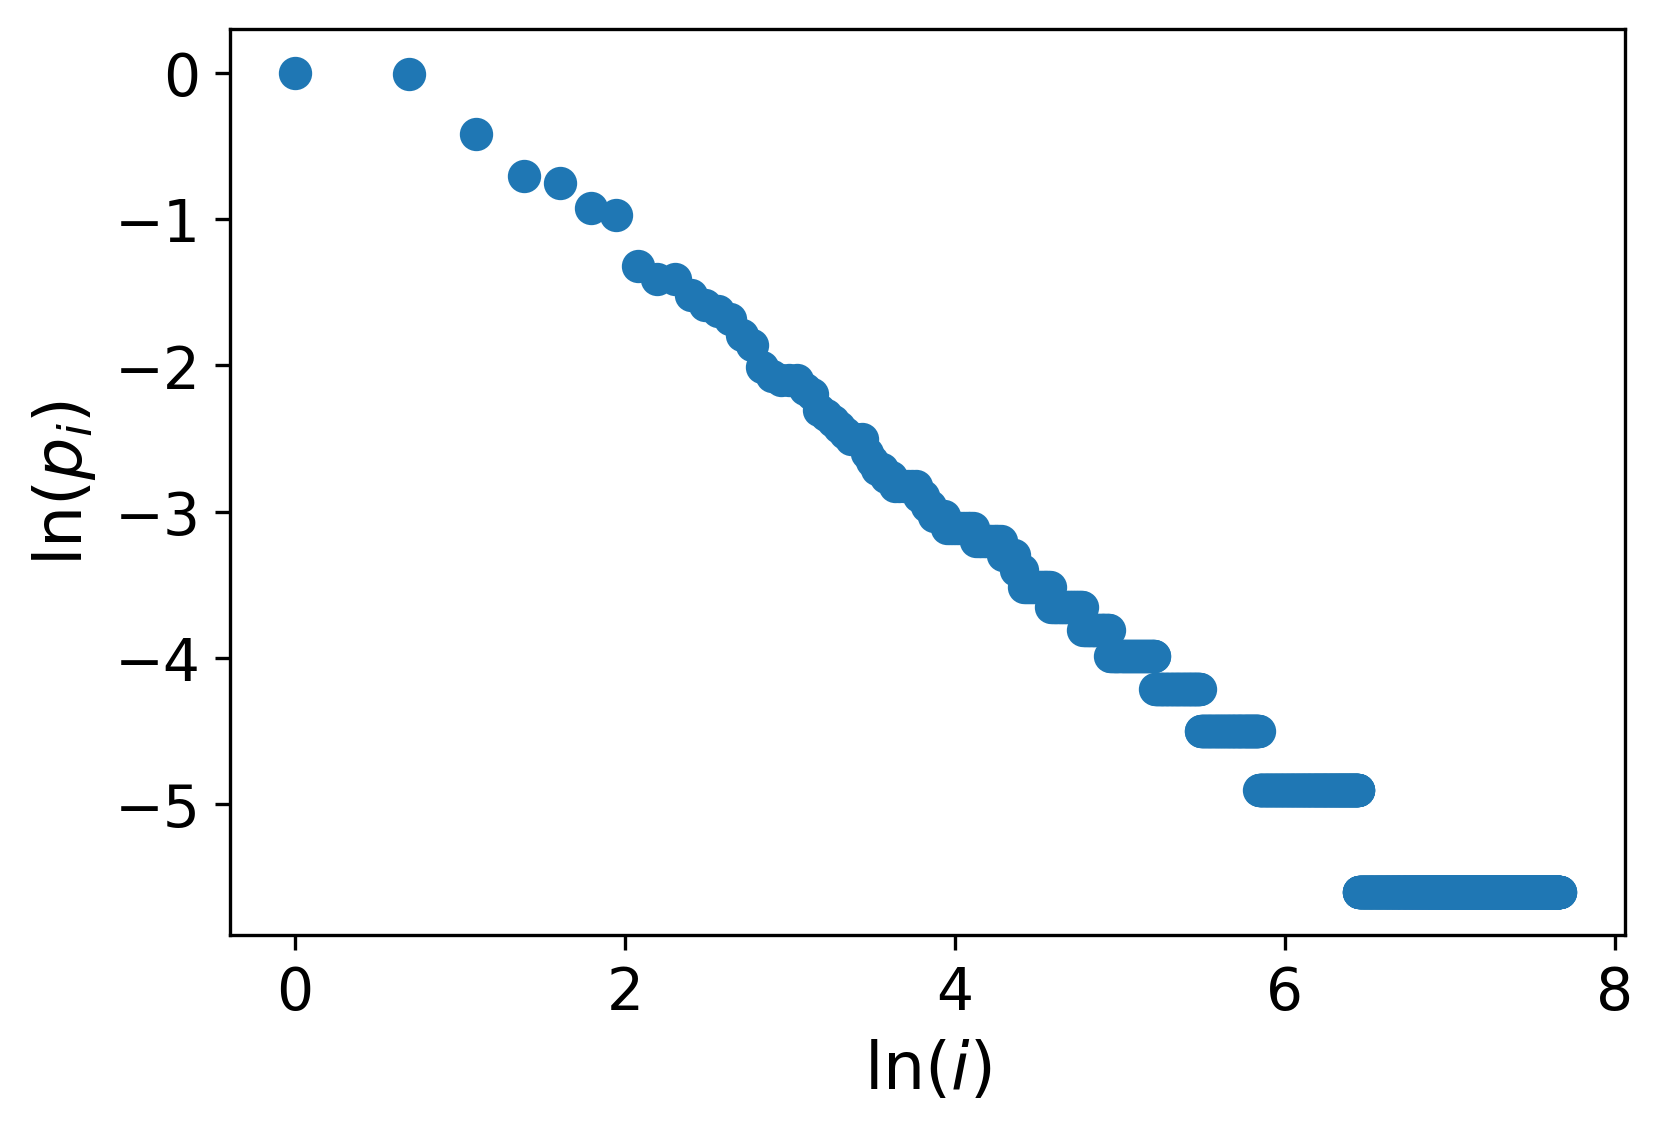
\includegraphics[width=0.99\linewidth]{images/parlost.png}
            \caption{}
        \end{subfigure}
        \begin{subfigure}{0.32\textwidth}
            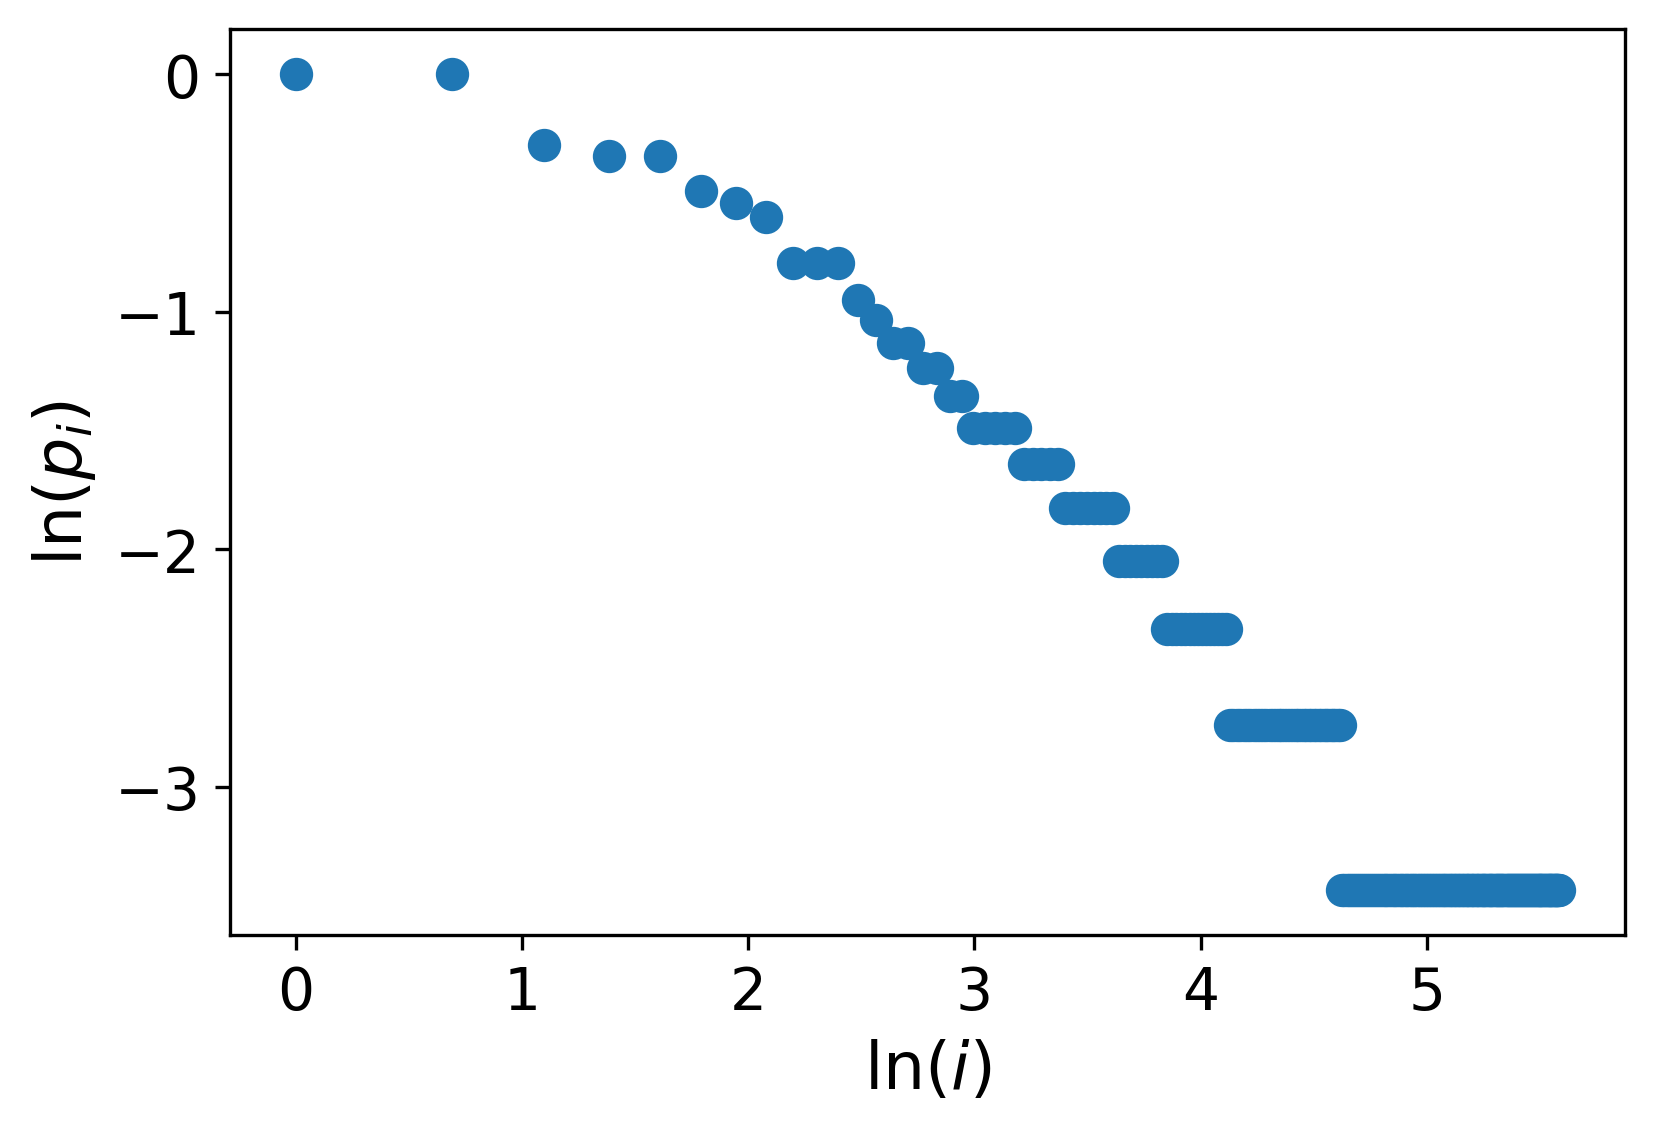
\includegraphics[width=0.99\linewidth]{images/alcapone.png}
            \caption{}
        \end{subfigure}
    \end{minipage}
    \caption{The results of analyzing six texts for adherence to Zipf's law: (a) \textcite{Moby-Dick}, (b) \textcite{Ulysses}, (c) \textcite{trump}, (d) \textcite{feynman}, (e) \textcite{paradiselost}, and (f) \textcite{capone}. Plots depict the natural log of word rank $i$ (by frequency) versus the natural log of word probability $p_i$; texts are Zipfian (i.e., follow Eq. \ref{eq:zipf}) to the extent that they are linear. The total number of words $N$, linear regression coefficient of determination $r^2$, and magnitude of the linear regression slope $|m|$ are given for each text on the left. Largely linear relationships ($r^2 \approx 1$) which mostly satisfying $\alpha = |m| \approx 1$ are revealed for (a) through (d), while (e) and (f) are presented as counterexamples.}
    \label{fig:plots}
\end{figure}
    
    \hspace*{0.5in} To build on the few examples provided in the previous paragraph, a survey of the existing linguistic research indicates a widespread agreement of language with Zipf's law. \textcite{large_scale_english} apply strict analyses to over $30000$ English texts found on Project Gutenburg to test for a few slightly different forms of Zipf's law and find agreement in over $40\%$ of the examined cases, an impressively high number when considering their stringent statistical significance requirement of $\alpha = 0.05$ for agreement (not to be confused with the exponent $\alpha$ appearing in Eqs. \ref{eq:zipf}, \ref{eq:log}). Moving beyond just English, \textcite{seven_lang} find a collection of $91$ smaller texts across seven languages adhere to Zipf's law, and \textcite{fifty_lang} examine samples with over $80000$ words in $50$ distinct languages and similarly confirm the presence of Zipf's law (while the latter paper does additionally identify a subtle three-segment structure in the rank-probability relationship on top of the basic Zipfian pattern). \textcite{esperanto} even identify that the constructed language Esperanto obeys Zipf's law to an extent comparable to other natural languages. In conjunction, this literature suggests the validity of Zipf's law as a universal, inter-language phenomenon.
    
    \hspace*{0.5in} Given the evidence for Zipf's law in language samples, I now turn my attention to potential underlying reasons for this behavior, beginning with a statistical argument. In particular, \textcite{taylor_zipf} argue that Zipf's law emerges as a natural approximation to arbitrary word probability distributions. To show this, he invokes the result from information theory which claims that events with probability $p$ possess an ``information measure'' of $x = -\ln(p)$ (also yielding $p = e^{-x}$), and considers an arbitrary word cumulative probability distribution (CPD) $\phi(x)$, taken as a function of information measure. Such a function gives the probability of words with information less than or equal to $x$ occurring, so if $n$ unique words exist in a text then $n \cdot \phi(x)$ gives the number of words with lower (or equal) associated information (or, equivalently, equal or higher probability) than $x$, or in other words, the rank $i$ of $x$ among unique words by frequency. By computing the first-order Taylor expansion around an information value $x_0 = -\ln(p_0)$ with rank $i_0 = n\phi(x_0)$, and using the linear approximation $\ln(1 + x) \approx x$, the following can be derived.
    \begin{align*}
        \phi(x) &\approx \phi(x_0) + \phi'(x_0)(x - x_0) \Longrightarrow \ln\left(\frac{\phi(x)}{\phi(x_0)}\right) \approx \ln\left(1 + \frac{\phi'(x_0)}{\phi(x_0)}(x - x_0)\right)\\
        &\Longrightarrow \ln\left(\frac{\phi(x)}{\phi(x_0)}\right) \approx \frac{\phi'(x_0)}{\phi(x_0)}(x - x_0) \Longrightarrow \ln\left(\frac{i}{i_0}\right) \approx -\frac{\phi'(x_0)}{\phi(x_0)}\Big(\ln(p) - \ln(p_0)\Big)\\
        &\Longrightarrow \ln\left(\frac{p}{p_0}\right) \approx -\frac{\phi(x_0)}{\phi'(x_0)}\ln(i) + C
    \end{align*}
    Here, $C$ is just a constant dependent upon the fixed values $i_0$, $\phi(x_0)$, $\phi'(x_0)$: what is important is that, if we take $p_0$ to be the probability of the most frequent word, our arbitrary, assumption-free CPD $\phi$ has led us naturally to Eq. \ref{eq:zipf} and Zipf's law, suggesting that this linguistic phenomenon is but a special case of a broader probabilistic effect. Other authors take similar stances: \textcite{random_words_zipf}, for example, seeks to show that Zipf's law inevitably arises statistically from the near-universal human language process of assembling words from finite alphabets. However, I claim that these types of mathematical arguments should be treated with care, as they invoke substantial approximation. For example, in direct response to the previous reference, \textcite{not_random_words_zipf} argue that statistical Zipf's laws derivations aren't sufficiently rigorous, and employ more thorough Monte Carlo-style experimentation to show that random texts do not manifest Zipf's law. Given this contention associated with the validity of the above statistical approaches, I want to introduce an alternative, more natural framework which seeks to explain Zipf's law.
    
    \hspace*{0.5in} In contrast with the statistical explanation, some linguists, including Zipf himself, have employed substantiations for Zipf's law which draw from economics and mathematics to characterize the principle as the outcome of some sort of optimization problem. In his book, \textcite{zipf} posits that his law arises from what he calls the principle of least effort, or the idea that individuals seek out the lowest average rate of probable or foreseen work. By constructing rhetorical devices including the ``Bell Analogy'' and the ``Tool Analogy''---wherein a demon is tasked with ringing bells at various distances in a certain organized way, and an artisan must complete tasks while maintaining and optimizing their equipment, respectively---using them to derive classical economic principles, and generalizing their scopes (e.g., equating human speakers with the demon and the artisan), Zipf's law is arrived upon as a corollary of both speakers and listeners simultaneously following the principle of least effort. Other researchers utilize similar ideas, albeit from slightly different angles: \textcite{graph} characterizes linguistic interactions as two-person (speaker and listener) games on mathematical graphs (networks of nodes and edges connecting them) which, when simulated, naturally lead to Zipf's law. Similarly, \textcite{physics} invokes the calculus of variations---a mathematical approach to finding the extrema of functionals, or operations which map functions to numbers---to extract Zipf's law from a principle of maximum efficiency. I argue that it is the resemblance of these optimization-based explanations for Zipf's law to foundational results in physics which works to distinguish them. One of the more significant achievements in the field of physics is the discovery that, from celestial dynamics to electromagnetic interactions, and from macroscopic kinematics to quantum mechanics, the physical behavior of our universe is governed by optimization laws, and least action principles in particular. For example, the idea of optimization---and the calculus of variations in particular---underlies Lagrangian mechanics, which arises from the principle of least action (action being a mysterious physical quantity usually given by the difference of kinetic and potential energy). Given that optimization appears to be stitched into the fabric of our reality, it seems natural, coherent, and logical that other domains, such as language, are explained by similar structures.
    
    \hspace*{0.5in} When investigating the behavior of word frequencies in language, one is confronted with a remarkably simple and global structure: Zipf's law. Within the dynamic use of the constantly evolving, organic entity which is human language, an undeniable mathematical pattern emerges and connects the frequency rank and probability of words which are often chosen by speakers or writers on the fly, and are hardly ever produced with the intent of preserving some higher order. This pattern manifests itself across languages and in all different kinds of linguistic environments, appearing to be, to some extent, a fundamental and universal property of human language. The study and investigation of this phenomenon and its origins, then, is necessarily an analysis of the intrinsic nature of language itself. Perhaps Zipf's law arises merely as an approximation or statistical by-product of the inherent properties of the variables under consideration or the alphabet-based structure of language, but I argue that a more thorough and satisfying answer arises from the idea that language operates in the very same way nature does: optimization. In the same way that our universe moves in a way that minimizes the action, we might produce language in a way that minimizes the effort of speaker and listener. Regardless, the true explanation for Zipf's law is still an open question, but one of the utmost importance. Beyond the profound linguistic implications, resolving Zipf's law has wide ramifications, as it turns out that the principle actually appears everywhere from earthquake frequencies, as explored by \textcite{earthquake}, to music, as indicated by \textcite{music}. Zipf's law is also useful: for example, \textcite{impersonation} discuss how Zipf's law can be exploited to enable impersonation detection on social media, pointing to the value associated with studying and understanding this effect. There may be more questions than answers at this point, but Zipf's law represents an important principle in both language and science at large, and warrants every effort expended for its study.
     
    \bigskip
    
    The source code and raw text used in this paper can be found at \texttt{https://github.com/sheride/zipf\_paper.}
\end{flushleft}

\newpage

%\bibliography{ref}
%\bibliographystyle{apalike}
\printbibliography

\end{document}
